%  Created by Branden Stone on 2015-01-15.
%  Copyright (c) 2015 Branden Stone. All rights reserved.
%--------------------------------------------------------
\documentclass{article}


%---------------------------
% Packages
%---------------------------
\usepackage{amssymb, amsmath, latexsym, amsfonts, amsthm, mathrsfs} % Standard packages that are nice to have.
\usepackage{amsrefs} % Allows for easy referencing and citations.
\usepackage{verbatim} % Needed for \begin{comment} \end{comment}.
\usepackage[text={6in,9in},centering]{geometry} % Defines the dimensions of the text body.
\usepackage[colorlinks=true]{hyperref} % Allows for use of hyperlinks.
%\usepackage[doublespacing]{setspace} % Makes the document double spaced.
\usepackage[pdftex]{graphicx} % Allows for \includegraphics
\usepackage{enumerate} % Allows for easy modification of lists

\renewcommand{\arraystretch}{1.5}

%----------------------------
% Title and Author
%----------------------------

\title{Math 390 Homework 6}
\author{Due Friday, March 11}
\date{}


%----------------------------
% Main Document Body
%----------------------------

\begin{document}


%-------------------------------------------------------------
% Front Matter: This is where you can add a table of contents,
% preface, list of figures, ETC. for this template we will 
% only create a title and author name with `\maketitle'
%-------------------------------------------------------------

\maketitle

\setlength{\parindent}{0em} % Sets indentation of new paragraph
\setlength{\parskip}{1em} % Sets space between paragraphs

%-------------------------------------------------------------
% Document Body: Essentially this is where you place the 
% content of your document. To use this template, just delete
% all of the text between here and the Bibliography Section.
% Then type whatever you desire.
%-------------------------------------------------------------


Solutions should be written \LaTeX\ or Markdown and converted to a PDF. You are encouraged to work with others
on the assignment, but you should write up your own solutions independently. This means no copy pasting. You should
reference all of your sources, including your collaborators. 

\begin{enumerate}

\item 
\begin{enumerate}
	\item Can $K_{3,4}$ be drawn on the projective plane with no edge crossings? Can $K_{4,4}$ be drawn on the projective plane with no edge crossings? Prove your answers. (Recall that if a nonplanar graph can be drawn on the projective plane with no edge crossings, then the drawing must satisfy $n-m+f=1$.)

	\item Can $K_{3,4}$ be drawn on the torus with no edge crossings? Can $K_{4,4}$ be drawn on the torus with no edge crossings. Prove your answers. (Recall that if a nonplanar graph can be drawn on the torus with no edge crossings, then the drawing must satisfy v − e + f = 0.)
\end{enumerate}


\item Consider the following graph:
\begin{center}
	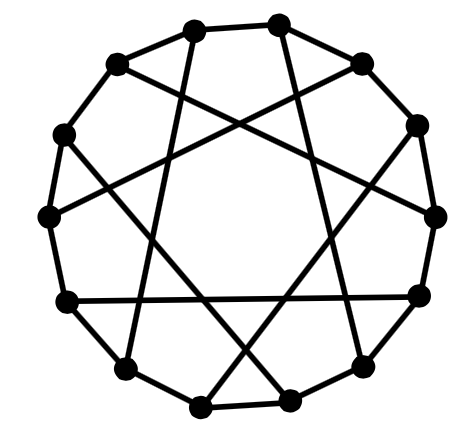
\includegraphics[width=.3\textwidth]{pic.png}
\end{center}
\begin{enumerate}
	\item Draw this graph on a torus without edge crossings. (Hint: Draw the cycle of length 14 so that it goes around the torus.)

	\item Create the dual graph to your answer to part (a). What graph is it?
\end{enumerate}

\end{enumerate}




\end{document}